\documentclass[12pt,a4paper,titlepage,openany]{report}
\usepackage{style}

\usepackage[slovene]{babel}
\usepackage[utf8]{inputenc}
\usepackage[T1]{fontenc}
\usepackage{lmodern}
\usepackage{csquotes}
\usepackage{hyperref}

\usepackage[
backend=biber,
style=numeric,
sorting=ynt
]{biblatex}

\addbibresource{bibliografija.bib}


% Glava dokumenta:

\fancyhf{}
\lhead[]{{\fontsize{9.3}{12}\selectfont
Rozman M. Razpoznavanje gibanja na osnovi elektroencefalografije.\\
\noindent Univerza na Primorskem, Fakulteta za matematiko, naravoslovje in informacijske tehnologije, 2024}}
\chead[]{\fancyplain{}{}}
\rhead[]{\fancyplain{\thepage}
{\thepage}}
\cfoot[]{\fancyplain{}{}}
\lfoot[]{\fancyplain{}{}}
\rfoot[]{\fancyplain{}{}}
\normalsize

%%%%%%%%%%%%%%%%%%%%%%%%% ZAČETEK DOKUMENTA %%%%%%%%%%%%%%%%%%%%%%%%%%%%%%%%%%%%%%%%%%5

%%%%%%%%%%%%%%%%%%%%%%%%% Naslovna stran %%%%%%%%%%%%%%%%%%%%%%%%%


\begin{document}
\pagenumbering{Roman}
\pagestyle{empty}
\begin{center}
\noindent \large UNIVERZA NA PRIMORSKEM\\
\large FAKULTETA ZA MATEMATIKO, NARAVOSLOVJE IN\\
INFORMACIJSKE TEHNOLOGIJE


\normalsize
\vspace{6cm}
Zaključna naloga\\
\textbf{\large Razpoznavanje gibanja na osnovi elektroencefalografije}\\
\normalsize
(Movement recognition based on electroencephalography)\\
\end{center}

\begin{flushleft}
\vspace{5cm}
\noindent Ime in priimek: Marko Rozman
% v zgornjo vrstico dopišite ime in priimek študenta
\\
\noindent Študijski program: Računalništvo in informatika
% v zgornjo vrstico dopišite ime študijskega programa
\\
\noindent Mentor: doc. dr. Peter Rogelj 
% v zgornjo vrstico dopišite akademski naziv, ime in priimek mentorja

\end{flushleft}

\vspace{4cm}
\begin{center}
\large \textbf{Koper, Julij 2024}
% dopišite mesec in leto oddaje zaključne naloge
\end{center}
\newpage

\pagestyle{fancy}
%%%%%%%%%%%%%%%%%%%%%%%%%%%%%%% Ključna dokumentacijska informacija (slo in ang) %%%%%%%%%%%

\section*{Ključna dokumentacijska informacija}

\medskip
\begin{center}
\fbox{\parbox{\linewidth}{
\vspace{0.2cm}
\noindent
Ime in PRIIMEK: Marko ROZMAN\vspace{0.5cm}\\
Naslov zaključne naloge: Razpoznavanje gibanja na osnovi elektroencefalografije\vspace{0.5cm}\\
Kraj: Koper\vspace{0.5cm}\\
Leto: 2024\vspace{0.5cm}\\
Število listov: 34\hspace{2cm} Število slik: 15\hspace{2.6cm} Število tabel: 2\hspace{2cm}\vspace{0.5cm}\\
Število referenc: 14\vspace{0.5cm}\\
Mentor: doc. dr. Peter Rogelj\vspace{0.5cm}\\
Ključne besede: elektroencefalografija, Grangerjev index vzročnosti, kompleksni Pearsonov korelacijski koeficient, nevronska mreža, razvrščanje  \vspace{0.5cm}\\
{\bf Izvleček:}\\
Namen naloge je spoznati metode za razpoznavanje gibanja na osnovi elektroencefalografije. Gibanje smo razpoznavali iz podatkov EEG Motor Movement/Imagery Dataset in podatkov ki smo jih posneli sami na napravi Cognionics Quick-20. Iz posnetkov smo izračunali matrike povezljivosti z Grangerjevim indexom vzorčnosti in kompleksnim Pearsonovim korelacijskim koeficientom ki smo jih nato razvrstili z različnimi algorimi, vključno z nevronskimi mrežami. Naši rezultati kažejo da je v določenih primerih razvrščanje bolj točno z uporabo kompleksnega Pearsonovega korelacijskega koeficienta. 
\vspace{0.2cm}
}}
\end{center}

\newpage

\section*{Key words documentation}

\medskip

\begin{center}
\fbox{\parbox{\linewidth}{
\vspace{0.2cm}
\noindent
Name and SURNAME:\vspace{0.5cm}\\
Title of final project paper:\vspace{0.5cm}\\
Place:\vspace{0.5cm}\\
Year:\vspace{0.5cm}\\
Number of pages:\hspace{1.6cm} Number of figures:\hspace{2.2cm} Number of tables:\vspace{0.5cm}\\
Number of appendices:\hspace{0.6cm} Number of appendix pages:\hspace{0.8cm}Number of references:\vspace{0.5cm}\\
Mentor: title~First Name~Last Name, PhD\vspace{0.5cm}\\
% opomba: za "title" vpišite eno od naslednjega:
% Assist.~Prof. (če je naziv docent),
% Assoc.~Prof. (če je naziv izredni profesor),
% Prof. (če je naziv profesor)
Co-Mentor:\vspace{0.5cm}\\
Keywords:\vspace{0.5cm}\\
Math.~Subj.~Class.~(2010):\vspace{0.5cm}\\
{\bf Abstract:}
\vspace{0.2cm}
}}
\end{center}




%%%%%%%%%%%%%%%%%%%%%%%%%%%%%%% Zahvala %%%%%%%%%%%%%%%%%%%%%%%%%%%%%%%%%%%%%

\newpage
\section*{Zahvala}
Iskreno se zahvaljujem svojemu mentorju, doc. dr. Petru Roglju, za neprecenljivo podporo in vodenje pri pisanju diplomske naloge. Njegova strokovna pomoč pri izbiri metod, implementaciji ter pisanju je bila ključnega pomena na vsakem koraku. Hvaležen sem za priložnost dela s fizično napravo in za redne konzultacije ob sredah, ki so pripomogle k jasnosti in uspešnosti mojega dela.

Prav tako se iz srca zahvaljujem prijateljem in družini za njihovo neomajno podporo in spodbudo skozi celoten proces.

%%%%%%%%%%%%%%%%%%%%%%%%%%%%% Kazala %%%%%%%%%%%%%%%%%%%%%%%%%%%%%%
\newpage

% Dodamo kazala (po potrebi):
\tableofcontents
\addtocontents{toc}{\protect\thispagestyle{fancy}}
\newpage
\listoftables
\addtocontents{lot}{\protect\thispagestyle{fancy}}
\newpage
\listoffigures
\addtocontents{lof}{\protect\thispagestyle{fancy}}
\newpage
% ker priloge niso oštevilčene, tudi pikic do številk strani (ki jih ni) ne izpišemo
\renewcommand{\cftdot}{}
\listofappendices
\thispagestyle{fancy}
\newpage

\chapter*{Seznam kratic}
\thispagestyle{fancyplain}
\begin{longtable}{@{}p{1cm}@{}p{\dimexpr\textwidth-1cm\relax}@{}}

\nomenclature{$EEG$}{electroencephalography}
\nomenclature{$MMID$}{Motor Movement/Imagery Dataset} 
\nomenclature{$PLI$}{phase lag index}
\nomenclature{$wPLI$}{weighted phase lag index}
\nomenclature{$k-NN$}{k nearest neighbours}
\nomenclature{$SVM$}{support vector machine}
\nomenclature{$CPCC$}{complex Pearson correlation coefficient}
\nomenclature{$GC$}{Granger causality}

\end{longtable}
\newpage

\normalsize

%%%%%%%%%%%%%%%%%%%%%%%%%%%%%%%%%% Poglavja: %%%%%%%%%%%%%%%%%%%%%%%%%%%%%%%%%%%%%

% Namig: Za večjo preglednost datoteke lahko vsebino vsakega poglavja shranite v poseben .tex dokument
% v isto mapo, kjer je shranjena osnovna .tex datoteka. Nato poglavja vstavite v dokument s klicem \include
% Primer: PrvoPoglavje.tex in DrugoPoglavje.tex vstavimo tako:
% \include{PrvoPoglavje}
% \include{DrugoPoglavje}

\chapter{Uvod}
\thispagestyle{fancy}
\pagenumbering{arabic}
Motivacija za raziskavo je bila ugotoviti, do kakšne mere je mogoče razpoznavanje gibanja v živo na osnovi analize možganske aktivnosti z meritvami elektronecefalografije (EEG) . Najprej smo podatke iz prosto dostopne zbirke podatkov s pomočjo knjižnice EEGLAB razdelili na nekaj različno dolgih epoh po dogodkih in jim zožili frekvenčne pasove. Iz vsake pridobljene zbirke podatkov smo izračunali matrike povezljivosti Grangerjevega indeksa vzročnosti in matrike povezljivosti kompleksnega Pearsonovega korelacijskega koeficienta. Na pridobljenih podatkih smo naučili nevronsko mrežo. Iz pridobljenih rezultatov smo se odločili za nadaljevanje razvoja na zbirki, ki je obetala najboljšo točnost. Da bi omogočili delovanje v realnem času smo implementirali nekaj že obstoječih funkcij iz knjižnice. Posneli smo podatke na napravi Cognionics Quick-20 in dodatno naučili nevronsko mrežo na naših podatkih za boljše razvrščanje.
\newpage
\section{Elektroencefalografija}
Elektroencefalografija je metoda za merjenje možganske električne aktivnosti. Meri električne potenciale na površini temena, ki jih deloma generira možganska aktivnost. V zadnjem stoletju so znanstveniki s pomočjo EEG pridobili vpogled v različne nevrološke bolezni. V zadnjem času pa se pojavlja interes za modeliranje EEG signalov in uporabo le-teh za nadzor fizičnih naprav (ang. Brain-Computer Interfacing). EEG signali so običajno razdeljeni v frekvenčna območja, ki odražajo različne spektralne vrhove in jih povezujemo z različnimi možganskimi procesi. Ta območja (Slika \ref{slika:eeg}) so običajno določena kot delta (1-4 Hz), theta (4-8 Hz), alpha (8-13 Hz), beta (13-20 Hz), in gamma (>20 Hz).
 \cite{nunezElectroencephalographyEEGNeurophysics2016}
 \begin{figure}[h]
    \begin{center}
    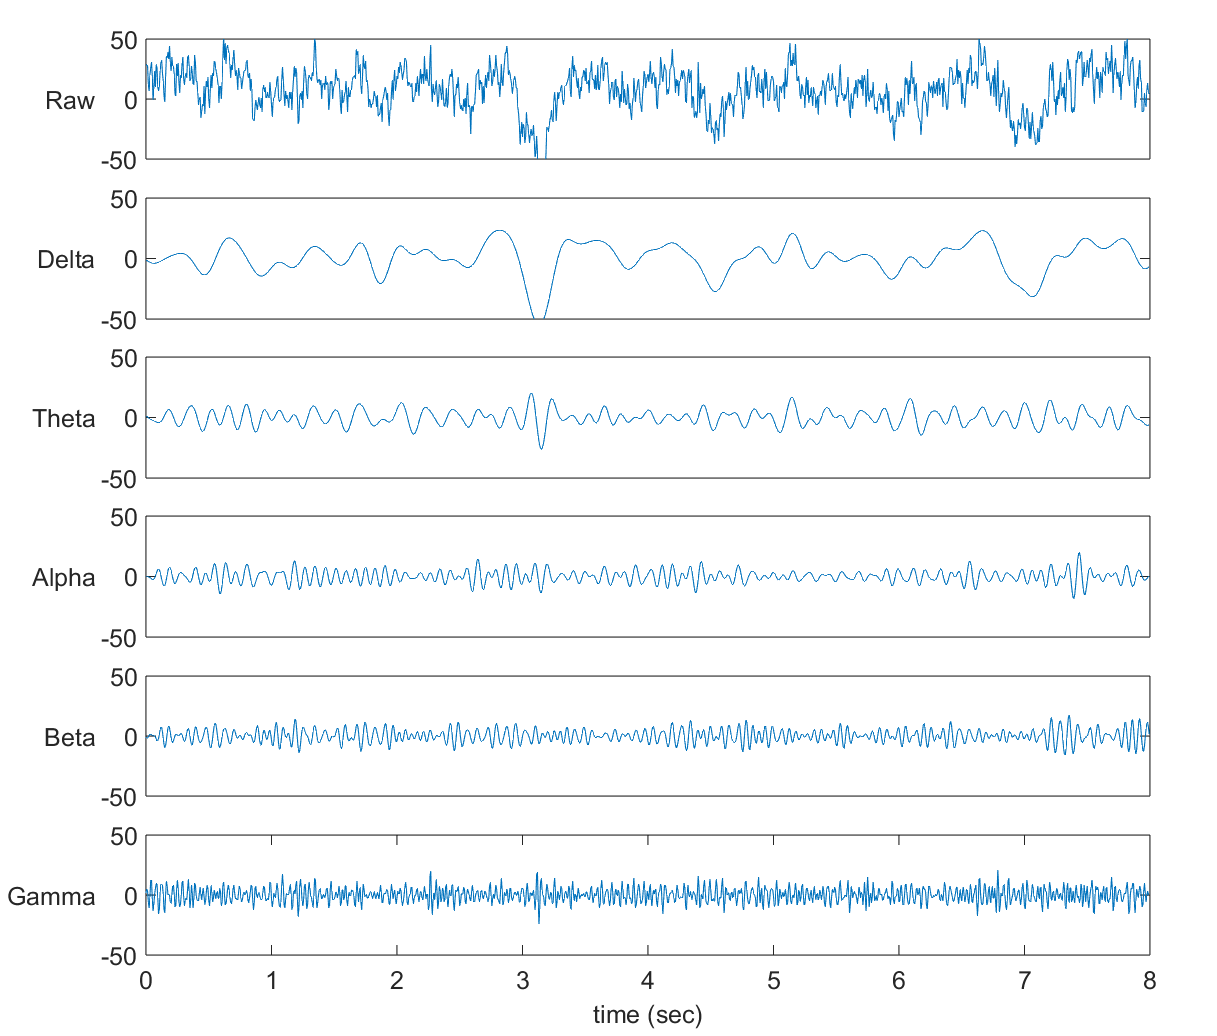
\includegraphics[width=1\linewidth]{slike/EEGSignals.png}
    \end{center}
    \caption[Frekvenčna območja EEG signala.]{Prvih 8 sekund EEG signala elektrode C3, osebe S001 serije R03. Od zgoraj navzdol po področjih: vsa skupaj, delta, theta, alpha, beta, gamma.}
    \label{slika:eeg}
    \end{figure}


\subsection{Mednarodni sitem 10-20 postavitve elektrod}
Mednarodni sistem 10-20 (slika \ref{slika:mednarodni_sistem_20}) standardizira mesta elektrod tako, da so te  nameščene v mrežo od naziona do iniona ter od desnega do levega sluhovoda v presledkih 10 in 20 odstotkov razdalje. Vsaka elektroda je označena s črko lokacije: $T$ -Temporal, $F$ -Frontal, $P$ -Parietal, $C$ -Central in $O$ -Occipital, ter s črko $Z$ za elektrode na sredini glave, lihimi številkami za levo polovico glave in sodimi za desno. \cite{klemTentwentyElectrodeSystem1999} Poleg mednarodnega sistema 10-20 za postavitev elektrod obstajajo tudi drugi sistemi, kot je na primer mednarodni sistem 10-10 postavitve elektrod. Podatki, snemani v živo, so bili pridobljeni po mednarodnem sistemu 10-20, medtem ko je bila podatkovna zbirka, uporabljena za učenje, snemana po prilagojenem mednarodnem sistemu 10-10 postavitve elektrod.
\begin{figure}[h]
    \begin{center}
    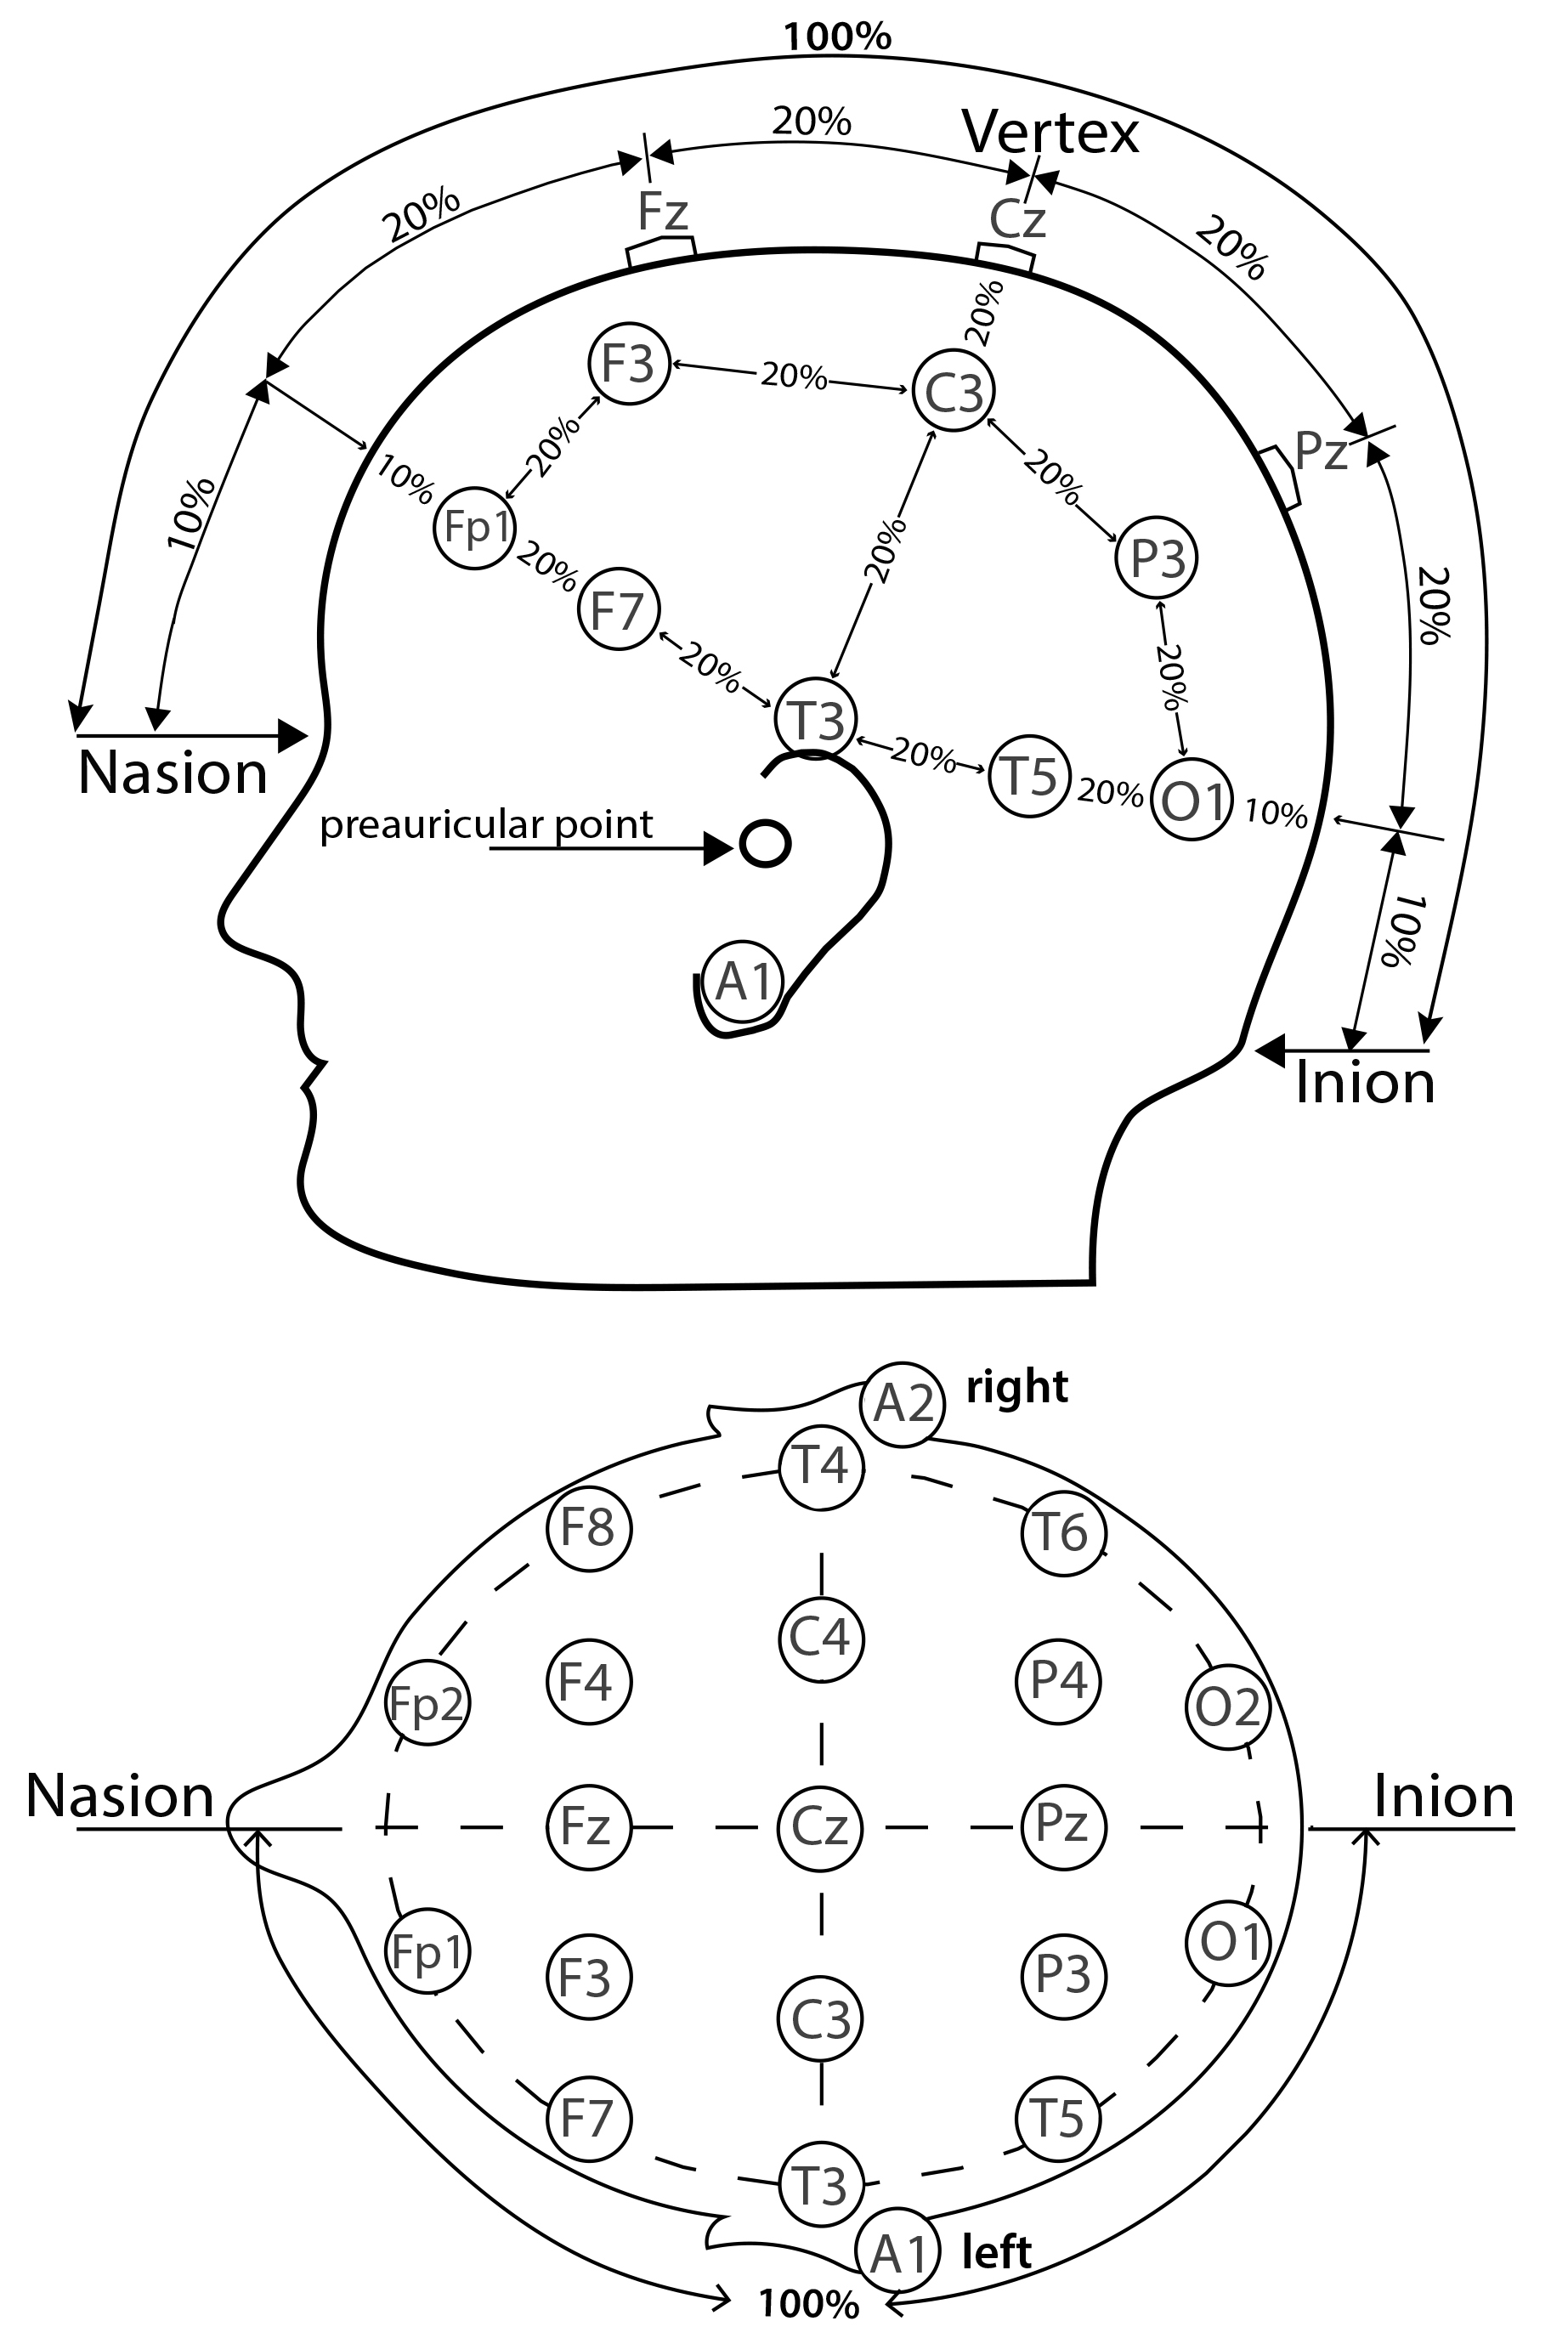
\includegraphics[width=0.5\linewidth]{slike/1020-diagram1.jpg}
    \end{center}
    \caption[Mednarodni sitem 10-20 postavitve elektrod.]{Prikaz postavitve elektrod po mednarodnem sitemu 10-20. Nameščene v mrežo od naziona do iniona in od levega do desnega sluhovoda v presledkih 10 in 20 odstotkov. \cite{ElectrodeArrangementAccording}}
    \label{slika:mednarodni_sistem_20}
    \end{figure}

\begin{figure}
        \begin{center}
        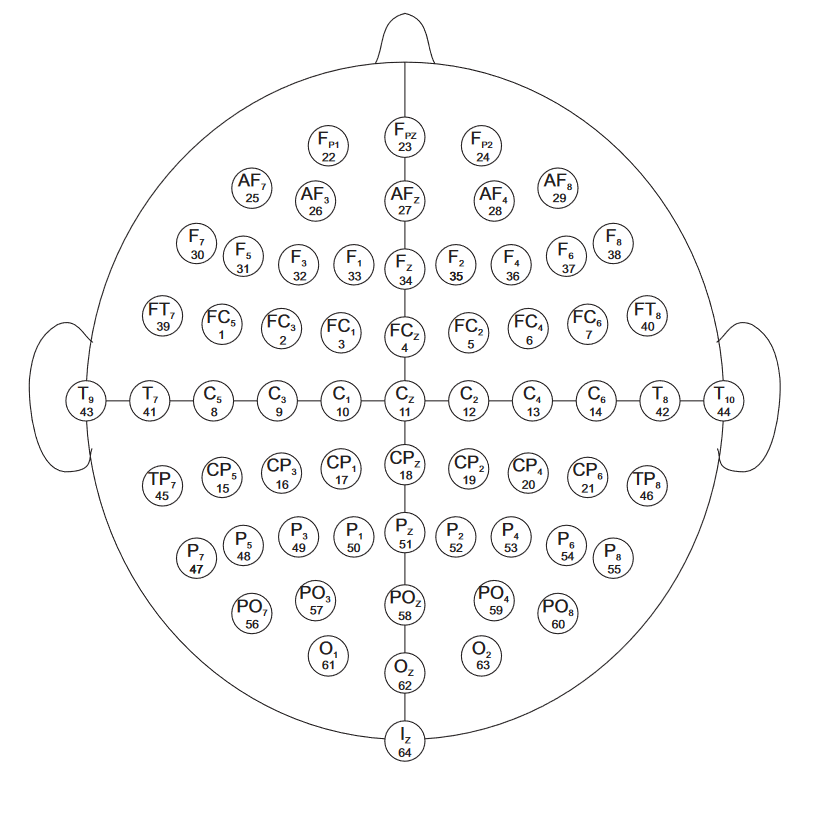
\includegraphics[width=1\linewidth]{slike/64electrodeSystem.png}
        \end{center}
        \caption[Mednarodni sitem 10-10 postavitve elektrod.]{Prikaz postavitve elektrod po mednarodnem sitemu 10-10.  \cite{HttpsWwwPhysionet}}
        \label{slika:mednarodni_sistem_10}
        \end{figure}

\newpage

\subsection{Cognionics Quick-20}
Cognionics Quick-20 (slika \ref{slika:quick_20}) je brezžična EEG naprava s suhimi elektrodami za raziskovalne namene. Ima 21 elektrod postavljenih po mednarodnem sitemu 10-20 za postavitev elektrod. Naprava je suhega tipa, kar pomeni, da pri uporabi elektrode gel ni potreben. Suhi tipi naprav so v primerjavi z mokrimi enostavnejši in udobnješi za uporabo ter omogočajo hitro nastavitev. Naprava je brezžična, z računalnikom jo povežemo preko USB vmesnika. \cite{DryEEGHeadset}

\begin{figure}[h!]
    \begin{center}
    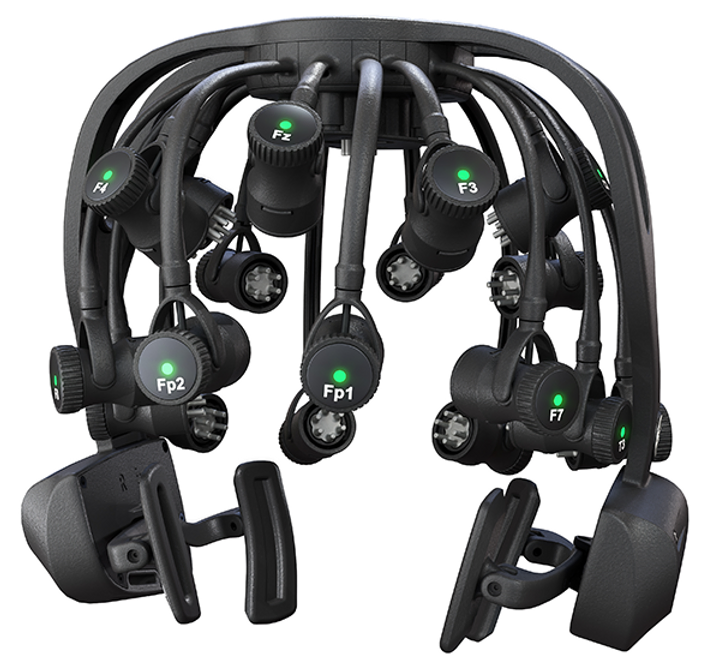
\includegraphics[width=0.5\linewidth]{slike/Cognionics Quick-20.png}
    \end{center}
    \caption[EEG naprava Cognionics Quick-20.]{EEG naprava Cognionics Quick-20. \cite{CognionicsQUICK20User}}
    \label{slika:quick_20}
    \end{figure}
\section{Možganska povezljivost}
Možganska povezljivost se nanaša na vzorce, nastale zaradi anatomskih povezav možganov, statistične odvisnosti ali interakcij med posameznimi deli možganov. Enote, med katerimi se meri povezljivost, so lahko različne: posamezni nevroni, nevronske populacije, ali pa kot v našem primeru regije možganske skorje. Možganska aktivnost je omejena s povezljivostjo, le-ta pa je zato ključnega pomena za razumevanje delovanja možganov. V grobem poznamo dve vrsti povezljivosti: strukturno in funkcijsko. Strukturna povezanost se nanaša na anatomsko povezanost različnih delov možganov. Funkcijska povezljivost pa se nanaša na to kako različni deli možganov med seboj komunicirajo oziroma sodelujejo.\cite{spornsBrainConnectivity2007} Funkcijsko povezljivost lahko nadaljnjo delimo na usmerjeno in neusmerjeno. V našem primeru je metoda Grangerjevega indeksa vzročnosti (GC) usmerjena, saj je vpliv elektrode $A$ na elektrodo $B$ drugačen kot vpliv elektrode $B$ na elektrodo $A$. Metoda kompleksnega Pearsonovega korelacijskega koeficienta (CPCC) pa je neusmerjena, saj nam njegova vrednost pove le o povezanosti para elektrod zato se pri njej ne ugotavlja smeri vpliva.
V izrazu Grangerjev indeks vzročnosti je vzorčnost zavajajoč termin, saj nam Grangerjev indeks vzročnosti nakazuje le, da en signal vpliva na drugega vendar sta lahko v določenih primerih obe meritvi odvisni od nečesa tretjega.


\chapter{Metode}

\section{Razvojno okolje}
Ves razvoj je potekal v programskem okolju MATLAB. Ta poleg samega programskega jezika vsebuje velik nabor že implementiranh funkcij, napredne aplikacije za strojno učenje in knjžnice ki omogočajo povezave z laboratorjskimi napravami. V njem sta ustvarjeni funkciji za računanje matric Grangerjevega indexa vzročnosti
in matric Kompleksnega Pearsonov korelacijskega koeficienta. V njem so ustvarjene nevronske mreže in uporabljeno je za ostale klasifikatorje. Prav tako smo v njem napisali funkcijo za zajemanje podatkov iz naprave Cognionics Quick-20, funkcijo ki v realnem času razpoznava gibanji.
    
\subsection{EEGLAB}
EEGLAB je interaktivna matlab orodjarna, za procesiranje in obdelavo elektrofizioloških podatkov. Omogoča rereferenciranje EEG signalov, izbiro določenih elektrod, deljenje podatkov na epohe glede na dogodke in filtriranje frekvenc. Omogoča interakcijo preko uporabniškega vmesnika. Vse akcije v vmesniku se prevedejo v ukaze ki jih lahko uporabimo v svoji kodi. Pri izdelavi naloge smo največ uporabljali funkcije branja .edf datotek, filtriranja frekvenc signalov in deljanja posnetkov na manjše dele.\cite{noauthor_eeglab_nodate}

\subsection{Lab streaming layer}
Lab streaming layer je odprtokodna vmesna programska oprema ki omogoča pošiljanje, prejemanje, sinhronizacijo in snemanje tokov podatkov. Omogoča enostavno povezovanje EEG naprave z programsko opremo MATLAB. Knjižnjico je potrebno prenesti in nato zgraditi na svojem računalniku.  \cite{noauthor_lsl-website_nodate}

\section{EEG Motor Movement/Imagery Dataset}
EEG Motor Movement/Imagery Dataset je prosto dostopna zbirka več kot 1500 eno in dve minutnih posnetkov 109 prostovoljcev ki opravljajo različne naloge. Za nas relevantni so posnetki serij 3, 5 in 7 v katerih prostovoljci stiskajo in sproščajo levo ali desno pest. Posnetki so shranjeni v formatu EDF+ ki vsebuje posnetke EEG in oznake dogodkov. Snemanje je bilo opravljeno s frekvenco 160Hz in 64 elektrodnim sistemom EEG.\cite{schalk_eeg_2009,schalk_bci2000_2004}

\section{Metode povezljivosti}
\subsection{Grangerjev index vzročnosti}
Grangerjev index vzročnosti je statistična metoda za preverjanje ali ena časovna vrsta nosi informacije o drugi. Metoda je bila razvita v šestdesedih letih devetnajstega stoletja za uporabo ekonomiji.

Za dve časovni vrsti $X_1$ in $X_2$, in $p$ kot število prejšnjih vrednosti ki jih upoštevamo pri računanju, lahko izračunamo $E_1$ in $E_1$ ki so napake pri predvidevanju naslednje vrednosti v vrsti $X_1$. V kolikor je varianca vrednosti $E_2$ manjša kot varianca vrednosti $E_1$ lahko predvidevamo da časovna vrsta $X_2$ nosi informacije o časovni vrsti $X_1$
\begin{align*}
X_1(t) &= \sum_{j=1}^{p} A_{1,j} X_1(t-j) + E_1(t)\\
X_1(t) &= \sum_{j=1}^{p} A_{2,j} X_1(t-j) + \sum_{j=1}^{p} A_{3,j} X_2(t-j) + E_2(t)
\end{align*}


\textcolor{red}{Mogoče razlaga kaj so A-ji. Ali so pravilno zapisani?}

\cite{seth_granger_2007}

\subsection{Kompleksni Pearsonov korelacijski koeficient}
Pearsonov korelacijski koeficient je najpogosteje uporabljen linearni korelacijski koeficient. Zanj smo se odločili saj v članku  \citetitle{sverko_complex_2022} avtorji pokažejo da vsebuje informacije PLI in wPLI ki sta dve najbolj pogosto uporabljeni metodi povezljivosti. V praksi nam pove, v kakšni meri sta fazi dveh signalov linearno povezani.

Ker želimo opazovati faze EEG signala, ga potrebujemo pretvoriti v analitični signal ki vsebuje informacijo o fazi. Zaradi sledeče transformacijo, ki je definirana samo na ozkih frekvenčnih pasovih potrebujemo signale EEG predhodno filtrirati. Analitični signal $X_a$ kjer $HT(X(t))$ označuje hilbertovo transformacijo signala $X$.
\begin{align*}
    X_a(t) = X(t) + i \cdot HT(X(t))
\end{align*}



\newpage
Za računanje Kompleksnega Pearsonovega korelacijskega koeficienta v našem primer lahko uporabimo naslednjo enačbo kjer sta $X_1$ in $X_2$ analitična signal dolžine $N$. $\overline{X_2(n)}$ pa konjugirana vrednost $X_2(n)$
\begin{align*}
r(X_1, X_2) &= \frac{\sum\limits_{n=1}^{N} X_1(n) \cdot \overline{X_2(n)}}{\sqrt{\sum\limits_{n=1}^{N} |X_1(n)|^2} \cdot \sqrt{\sum\limits_{n=1}^{N} |X_2(n)|^2}}.
\end{align*}
\textcolor{red}{Kaj predstavlja pika na koncu enačbe?}




\cite{sverko_complex_2022} 

\section{Klasifikacija}
Na pridobljenih matrikah povezljivosti smo preizkusili več vrst klasifikacije in sicer: odločitvena drevesa, metodo k najbližjih sosedov (k-NN), logistično regresijo, podporne vektorske stroje (SVM) in nevronske mreže.
\subsection{Classification learner}
Classification learner je aplikacija v Matlabu za enostavno klasifikacijo podatkov. Podpira različne metode klasifikacije, navzkrižno validacijo in uporabo različnih podatkov za gradnjo in testiranje modela. Z njo smo lahko hitro ocenili uspešnost računanja matric povezljivosti in primerjali delovanje različnih klasifikatorjev v primerjavi z našo nevronsko mrežo.
\newpage
\subsection{Nevronska mreža}
Nevronska mreža je sestavljena iz vhodne plasti za slike dimenzij 19x19x1, polno povezanega sloja s 100 nevroni, Leaky ReLU sloja, dropout sloja z 50\% verjetnostjo opustitve nevronov, polno povezanega sloja z 10 nevroni, GELU sloja, dropout sloja z 50\% verjetnostjo opustitve nevronov, polno povezanega sloja s tremi nevroni in Softmax sloja.
\begin{figure}[h!]
\begin{center}
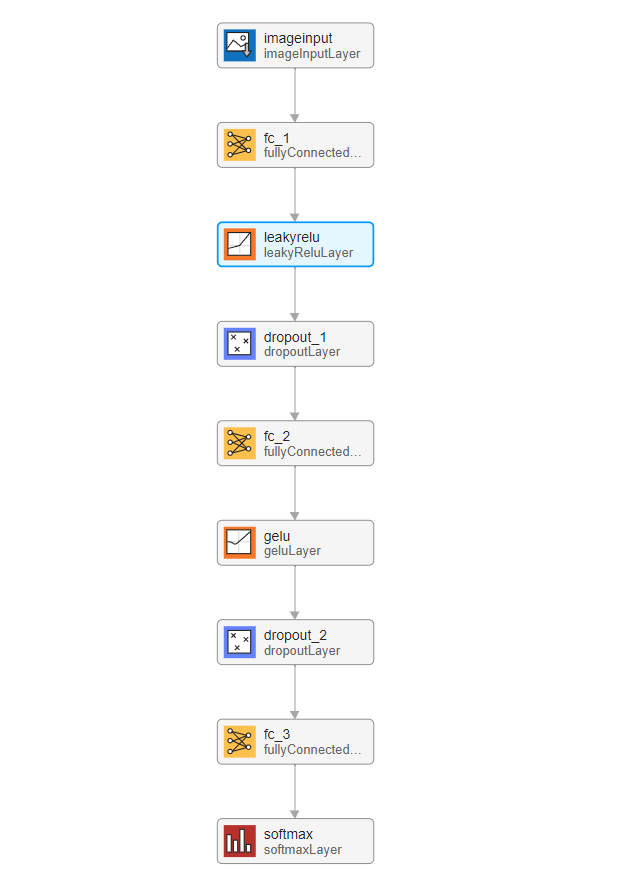
\includegraphics[width=0.5\linewidth]{slike/Neural network.png}
\end{center}
\caption{Nevronska mreža.}
\end{figure}

\section{Filtriranje}
Knjižnica EEGLAB vsebuje samo filtre z ničelno fazo, ki filtrirajo najprej in nato nazaj po času, kar v našem primeru ni primerno saj podatke prejemamo sekvenčno, zato smo podatke filtrirali s pomočjo Butterworthovega filtra ki vsebuje stanja. Ker pa filtra nista enakovredna, saj prvi ne spreminja faz drugi pa jih zamakne, uporabljena metoda CPCC pa deluje na zamikih faz, smo izvedli dodatno testiranje da smo preverili če pristop deluje enako učinkovito.

\section{Izbira metode povezljivosti}
\textcolor{red}{Mogoče že v rezultati?}\\
Ker je kompleksni Pearsonov korelacijski koeficient izračunan iz analitičnih signalov ga lahko definiramo samo za ozke frekvenčne pasove. Pri računanju Grangerjevega indexa vzročnosti te omejitve ni, tako da smo ga lahko računali na celotnem frekvenčnem območju do 45Hz. Prav tako se je pojavilo vprašanje koliko dolg epoho EEG signala bomo potrebovali za uspešno klasifikacijo, kot možnosti smo vzeli prvo sekundo, prvi dve sekundi, drugi dve sekundi in štiri sekunde. Natančnost klasifikacije smo ocenili z zgoraj navedeno nevronsko mrežo. Za najboljšo metodo se je izkazal kompleksni Pearsonov korelacijski koeficient na območju 13-30Hz z najdalšimi epohami, 4s.
\begin{figure}[h!]
    \begin{center}
    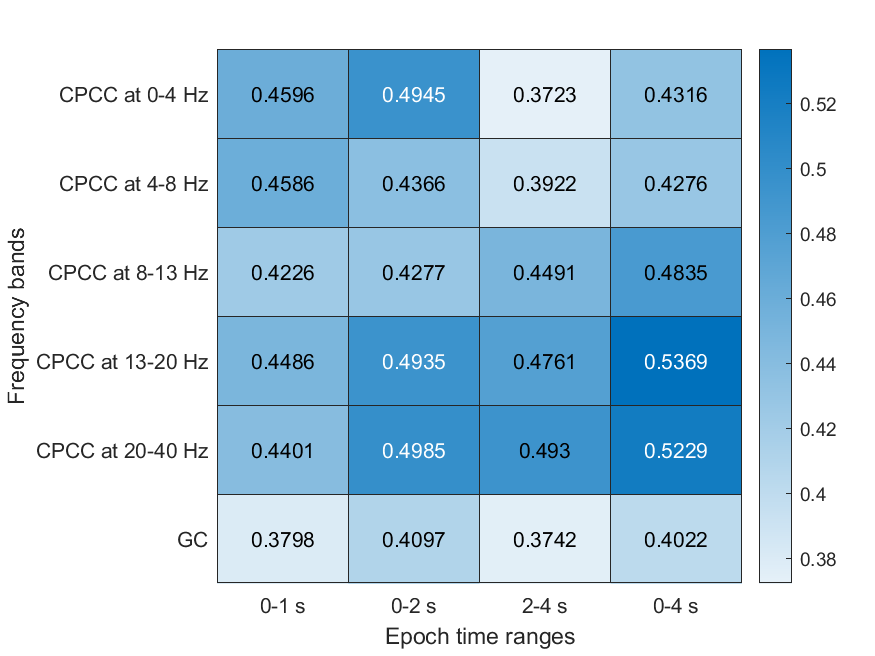
\includegraphics[width=0.5\linewidth]{slike/Comparison.png}
    \end{center}
    \caption{Primerjava območij in dolžin epoh.}
\end{figure}






\uppercaseChapter{Rezultati}
\thispagestyle{fancy}
\uppercaseSection{Točnost razvrščanja}
Pri interpretaciji točnosti razvrščanja stanj je potrebno upoštevati, da razvrščamo tri različna stanja, zato so že rezultati okoli 50\% bistveno nad nivojem naključnosti, ki je v primeru treh različnih stanj 33\%.
\uppercaseSection{Delitev podatkov}
Za končno raziskavo smo izbrali posnetke serij 3, 7 in 11 iz MMID. Vsaka serija vsebuje 109 posnetkov, vsak posnetek 30 primerov stanj, vse skupaj smo jih pridobili 9854. Primere stanj smo skrčili na enakomerno razporeditev z 2456 primeri vsakega stanja. Sami smo posneli nekaj minut posnetkov. Posneli smo vsega skupaj 250 primerov stanj, ki smo jih skrčili na enakomerno razporeditev, 62 primerov vsakega stanja. Za učenje nevronskih mrež smo uporabljali množice za učenje s 75\% podatkov in množice za testiranje s 25\% podatkov. Podatki so bili naključno razporejeni med učno in testno množico. Ker smo podatke delili naključno, se lahko različni posnetki stanj istega prostovoljca pojavijo v učni in testni množici. Pri dodatnem učenju mreže smo uporabili posnetke ene osebe za učenje in testiranje. To skupaj pomeni, da sistem ne deluje medosebno.


\uppercaseSection{Rezultati na MMID}
Za izbiro metode povezljivosti, načina filtriranja, dolžine epohe in frekvenčnega pasu smo uporabili podatkovno zbirko MMID.

\subsection{Izbira metode povezljivosti}
Ker je kompleksni Pearsonov korelacijski koeficient izračunan iz analitičnih signalov, ga lahko definiramo samo za ozke frekvenčne pasove. Pri računanju Grangerjevega indeksa vzročnosti te omejitve ni, zato smo ga lahko računali na celotnem frekvenčnem območju do 45Hz. Prav tako se je pojavilo vprašanje kako dolgo epoho EEG signala bomo potrebovali za uspešno razvrščanje. Kot možnosti smo vzeli prvo sekundo, prvi dve sekundi, drugi dve sekundi in prve štiri sekunde po dogodku. Točnost razvrščanja smo ocenili z zgoraj navedeno nevronsko mrežo. Za najboljšo metodo se je izkazal kompleksni Pearsonov korelacijski koeficient na območju 13-20 Hz z najdaljšimi epohami, 4s. Celotno območje primerjav je razvidno iz slike \ref{slika:primerjava_obmocij}.
\begin{figure}
    \begin{center}
    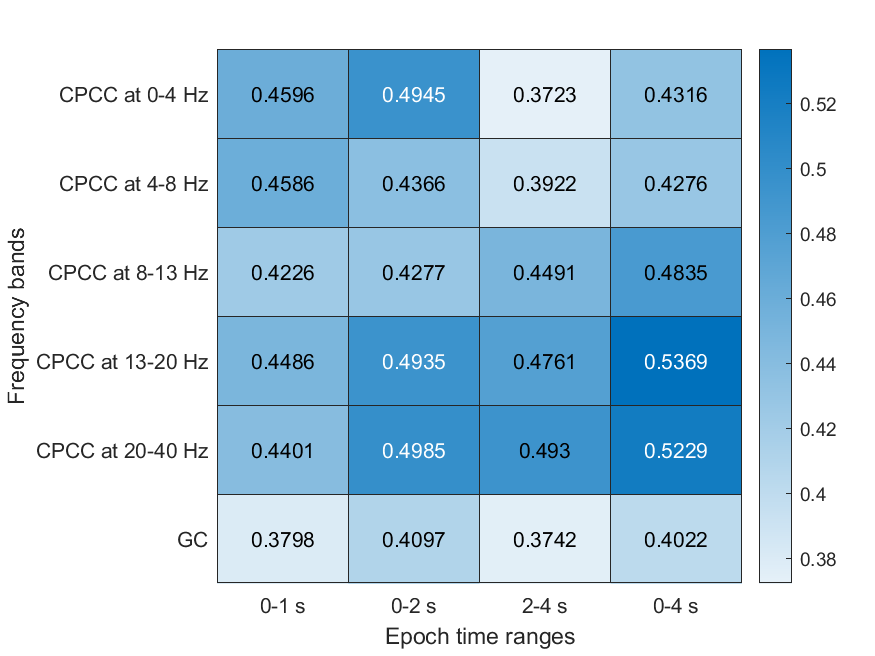
\includegraphics[width=1\linewidth]{slike/Comparison.png}
    \end{center}
    \caption[Točnost razvrščanja po frekvenčnih območjih in dolžini epoh.]{Točnost razvrščanja po frekvenčnih območjih in dolžini epoh za CPCC in GC. Od zgoraj navzdol: CPCC po pasovih delta, theta, alpha, beta in gamma. Spodnja vrstica: Grangerjev indeksa vzorčnosti. Epohe od leve proti desni: prva sekunda, prvi dve sekundi, drugi dve sekundi, prve štiri sekunde.}
    \label{slika:primerjava_obmocij}
\end{figure}

\newpage
\subsection{Izbira uporabljenih filtrov}
Knjižnica EEGLAB vsebuje samo filtre z ničelno fazo, ki filtrirajo naprej in nato nazaj po času, kar v našem primeru ni primerno, saj podatke prejemamo sekvenčno. Filtrov z ničelno fazo ni mogoče uporabiti v realnem času. Podatke smo želeli filtrirati s pomočjo Butterworthovega filtra, ki vsebuje stanja. Stanja nam omogočajo filtriranje sekvenčnih podatkov saj preprečijo napako na začetku filtra kjer le-ta potrebuje predpostaviti začetno staje vseh signalov 0. Ker filtra nista enakovredna, saj prvi ne spreminja faz drugi pa jih zamakne, uporabljena metoda CPCC pa deluje na zamikih faz, smo izvedli dodatno testiranje, da bi preverili ali pristop deluje enako učinkovito. Razvrščanje matrik, pridobljenih z Butterwothovim filtrom (slika \ref{slika:filter_matrika}b) v primerjavi z filtrom z ničelno fazo (slika \ref{slika:filter_matrika}a) je bilo primerljivo točno za frekvenčni pas beta (slika \ref{slika:primerjava_filtrov}) iz česar lahko sklepamo, da je filtriranje z Butterworthovim filtrom primerno.
\begin{figure}
    \begin{center}
    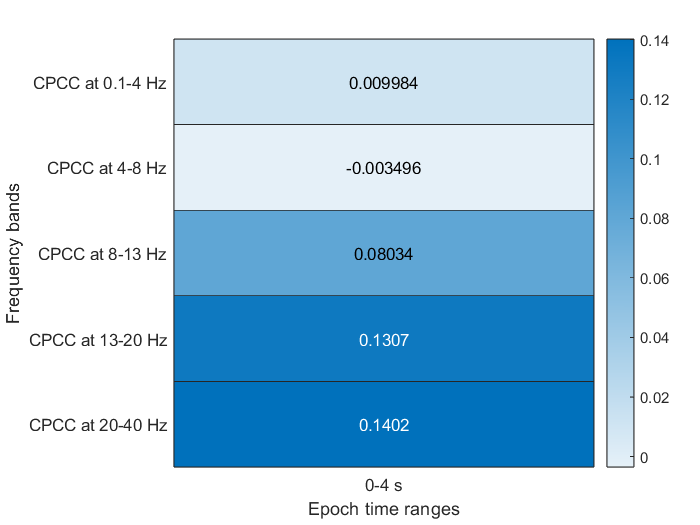
\includegraphics[width=1 \linewidth]{slike/ComparisonFilters.png}
    \end{center}
    \caption[Točnost razvrščanja glede na tip filtra in frekvenčno območje.]{Primerjava točnosti razvrščanja glede na tip filtra. Uporabljena metoda CPCC za epoho prvih štirih sekund za frekvenčne pasove delta, theta, alpha, beta in gamma. Razvrščanje z zgoraj navedeno nevronsko mrežo. Modra predstavlja Butterwothov filter, oranžna predstavlja filter z ničelno fazo.}
    \label{slika:primerjava_filtrov}
\end{figure}

\begin{figure}
    \begin{center}
    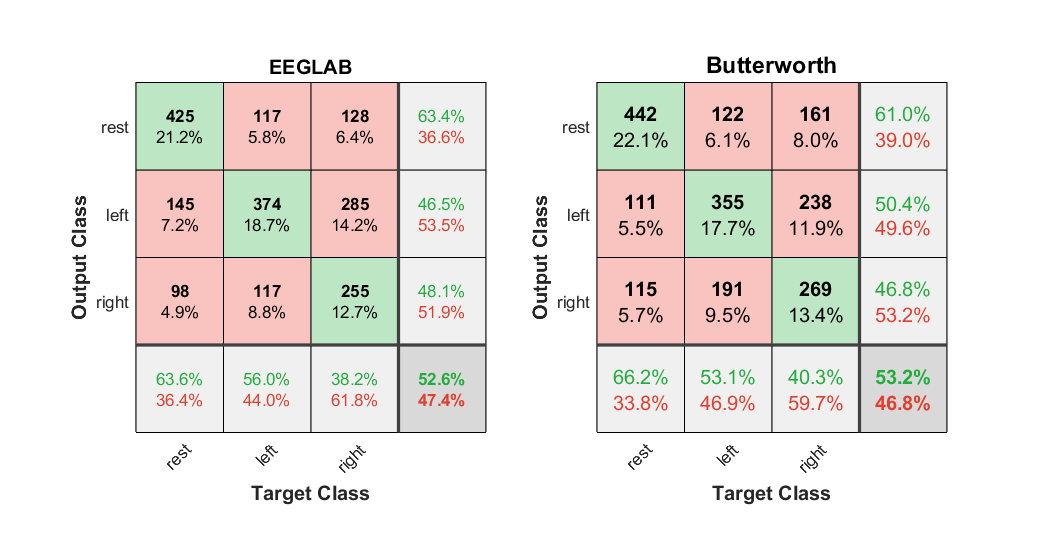
\includegraphics[width=1\linewidth]{slike/ComparisonFilters2.png}
    \end{center}
    \caption[Matriki zmede nevronskih mrež za frekvenčno območje beta.]{Matriki zmede nevronskih mrež, naučenih na podatkih, filtriranih s filtrom z ničelno fazo (levo) in Butterworthovim filtrom (desno). Uporabljena metoda CPCC za epoho prvih štirih sekund za frekvenčni pas beta. V zelenih poljih vidna točnost za posamezna stanja. Od zgoraj navzdol: stanje mirovanja, skrčena leva pest, skrčena desna pest.}
    \label{slika:filter_matrika}
    \end{figure}

\subsection{Rezultati z okoljem Classification Learner}
Z uporabo aplikacije Clasifiacation Learner smo testirali več načinov razvrščanja. Iz rezultatov predstavljenih v tabeli \ref{tabela:primerjava_tocnosti} lahko razberemo, da so se za najbolj uspešne izkazale metode podpornih vektorjev (SVM), vendar so te metode računsko zahtevne, kar otežuje izvedbo v realnem času. Dober kandidat bi lahko bila odločitvena drevesa, saj so enostavna za učenje in interpretacijo, vendar so le ta dosegla 41\% točnost. Nevronske mreže ki jih podpira aplikacija so enostavne, vendar pa je njihova interpretacija težja.  Dosegle so 49\% točnost.
\begin{table}
\caption{Točnost vseh testiranih metod razvrščanja v aplikaciji Clasification Learner.}
\vspace{3mm}
\centering
\begin{tabular}{|l|l|c|}
\hline
vrsta razvrščanja & metoda & točnost [\%] \\
\hline SVM&Quadratic SVM&53\\
\hline SVM&Linear SVM&53\\
\hline SVM&Medium Gaussian SVM&53\\
\hline Ensemble&Subspace Discriminant&53\\
\hline SVM&Cubic SVM&52\\
\hline Kernel&SVM Kernel&52\\
\hline Kernel&Logistic Regression Kernel&52\\
\hline SVM&Coarse Gaussian SVM&50\\
\hline Efficient Logistic Regression&Efficient Logistic Regression&49\\
\hline Neural Network&Wide Neural Network&49\\
\hline Neural Network&Medium Neural Network&47\\
\hline Efficient Linear SVM&Efficient Linear SVM&46\\
\hline Neural Network&Trilayered Neural Network&45\\
\hline Neural Network&Bilayered Neural Network&45\\
\hline Naive Bayes&Kernel Naive Bayes&45\\
\hline Neural Network&Narrow Neural Network&45\\
\hline Ensemble&Bagged Trees&44\\
\hline KNN&Coarse KNN&44\\
\hline Ensemble&Boosted Trees&43\\
\hline Ensemble&RUSBoosted Trees&42\\
\hline Tree&Medium Tree&41\\
\hline Tree&Fine Tree&41\\
\hline KNN&Cosine KNN&41\\
\hline Tree&Coarse Tree&41\\
\hline KNN&Medium KNN&40\\
\hline KNN&Weighted KNN&40\\
\hline Ensemble&Subspace KNN&40\\
\hline KNN&Cubic KNN&40\\
\hline KNN&Fine KNN&38\\
\hline SVM&Fine Gaussian SVM&37\\

\hline
\end{tabular}

\label{tabela:primerjava_tocnosti}
\end{table}

\begin{figure}
    \begin{center}
    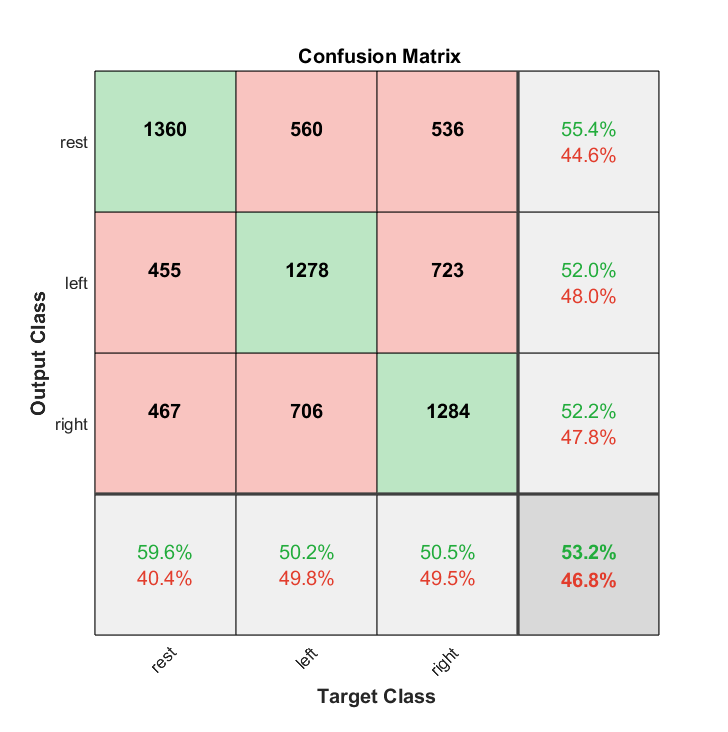
\includegraphics[width=0.8\linewidth]{slike/ConfusionSVM.png}
    \end{center}
    \caption[Matrika zmede metode Quadratic SVM.]{Matrika zmede metode Quadratic SVM. V poljih vidno število stanj. Od zgoraj navzdol: stanje mirovanja, skrčena leva pest, skrčena desna pest.}
    \label{slika:SVM_matrika}
    \end{figure}

\subsection{Rezultati z uporabo lastne nevronske mreže}
Nato smo poskusili z zgoraj navedeno nevronsko mrežo, ki razvršča matrike povezljivosti. Mreža je dosegla enako točnost kot metode iz aplikacije Clasification Learner in sicer 52\%. Če primerjamo matriko zmede nevronske mreže z matriko zmede metode SVM (sliki \ref{slika:nevronska_mreza_matrika} in \ref{slika:SVM_matrika} ), opazimo, da obe metodi bolj natančno razlikujeta stanje mirovanja od obeh stanj gibanja, medtem ko je razlikovanje med stanji gibanja med seboj manj natančno.

\begin{figure}
\begin{center}
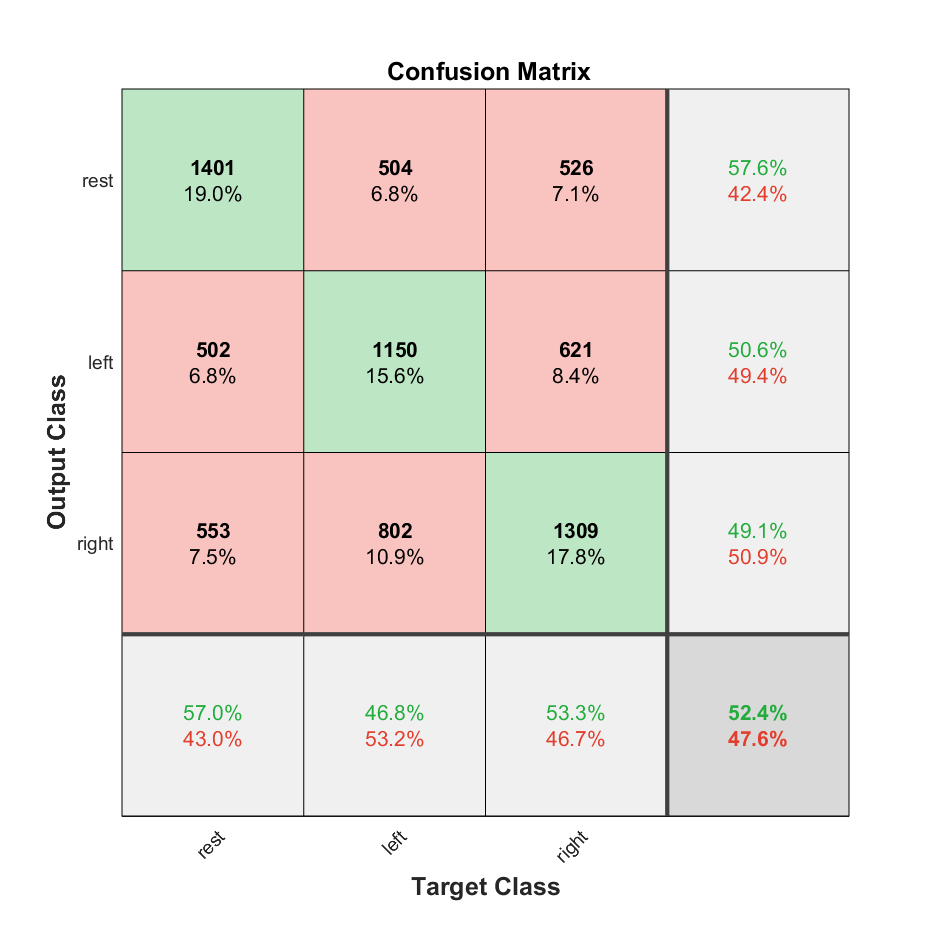
\includegraphics[width=0.8\linewidth]{slike/Confusion_13-20Hz_0s-4s.png}
\end{center}
\caption[Matrika zmede lastne nevronske mreže.]{Matrika zmede lastne nevronske mreže. V zelenih poljih vidna točnost za posamezna stanja. Od zgoraj navzdol: stanje mirovanja, skrčena leva pest, skrčena desna pest.}
\label{slika:nevronska_mreza_matrika}
\end{figure}



\uppercaseSection{Rezultati na lastnih podatkih}
Da bi se približali delovanju v realnem času, smo nevronsko mrežo dodatno naučili na naših podatkih. Zaradi različnih pogojev snemanja in natančnosti naprav, na katerih so podatki bili posneti, točnost razvrščanja pričakovano padla. Dosegli smo 43\% točnost. Ker nimamo velikega števila posnetkov smo uporabili petkratno prečno preverjanje. 
\begin{figure}
\begin{center}
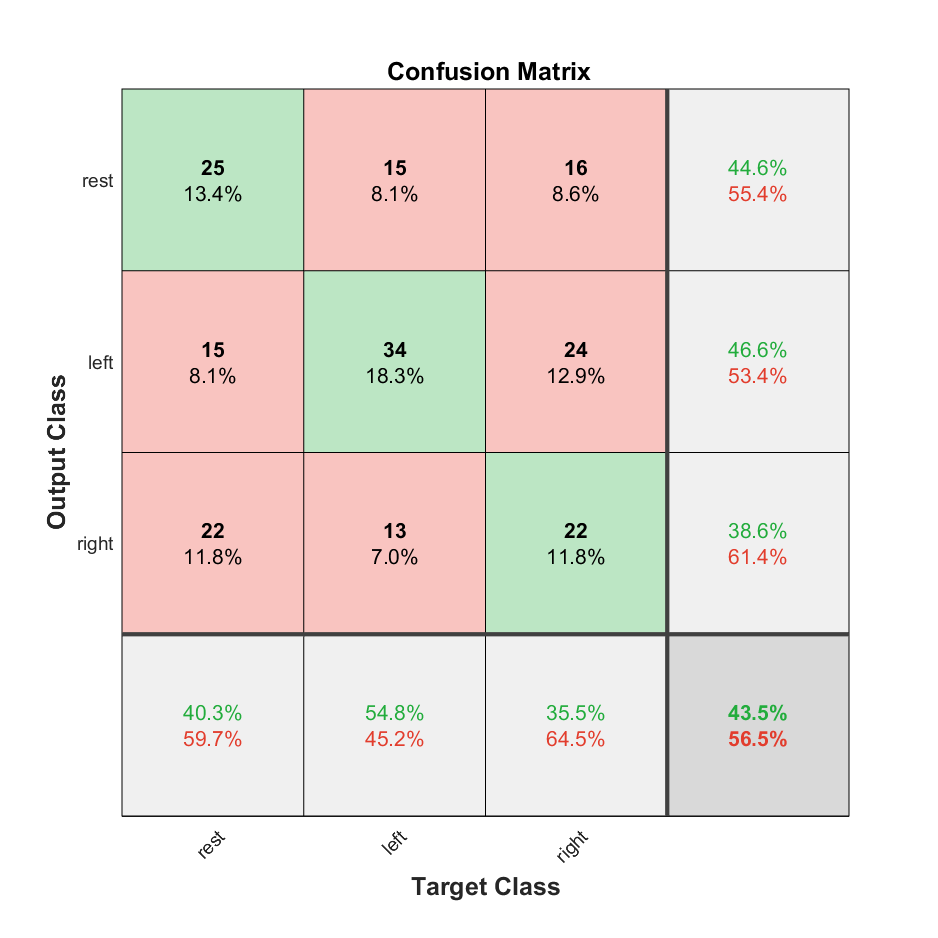
\includegraphics[width=0.8\linewidth]{slike/Confusion_13-20Hz_0s-4s_retrained.png}
\end{center}
\caption[Matrika zmede dodatno naučene nevronske mreže.]{Matrika zmede nevronskih mrež dodatno naučenih na naših podatkih.}
\end{figure}


\uppercaseSection{Sprotno razpoznavanje}
Po razvoju pristopov na zbirkah podatkov smo implementirali sprotno razpoznavanje. Za prenos podatkov iz naprave Quick-20 v okolje MATLAB smo uporabili programsko opremo Lab Streaming Layer. V okolju MATLAB smo podatke združevali in iz njih vsako sekundo izračunali matriko povezljivosti z metodo CPCC za frekvenčno območje beta, filtrirano z Butterwithovim filtrom. Matriko povezljivosti smo razvrstili in rezultat razvrščanja izpisali na zaslon. Na natančnost sprotnega razvrščanja matrik povezljivosti ene osebe vpliva veliko dejavnikov. Nanj vpliva razpoloženje osebe, namestitev naprave, sam dogodek, ki ga razvrščamo, pa tudi motnje v okolju, ki vplivajo na osebo in napravo. Točnosti razvrščanj nismo natančno izmerili, ocenjujemo pa, da je nižja od tiste, ki smo jo dosegli na prej posnetih podatkih. Kljub temu je iz rezultatov razvidno, da je klasifikacija gibanja v realnem času mogoča.

\begin{figure}
    \begin{center}
    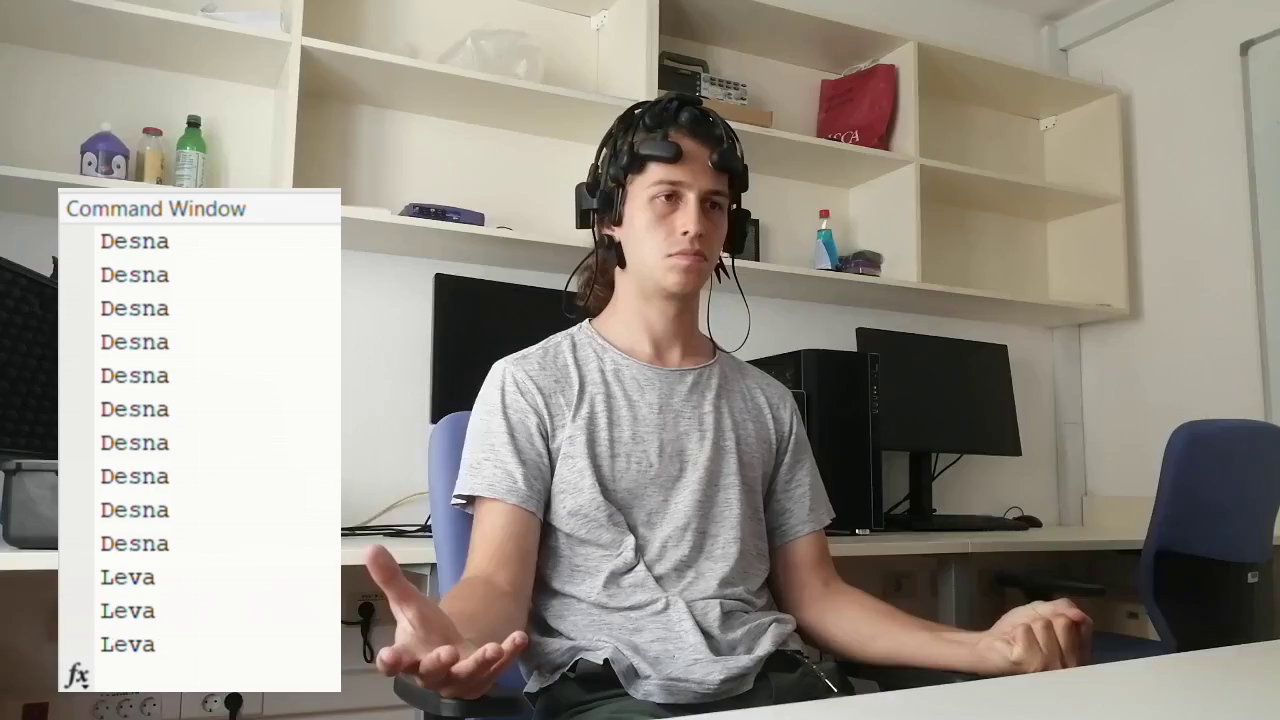
\includegraphics[width=1\linewidth]{slike/razpoznavanje.png}
    \end{center}
    \caption[Prikaz sprotnega razpoznavanja]{Prikaz sprotnega razpoznavanja. Dodan izpis razvrščanja iz okolja MATLAB.}
    \end{figure}





\chapter{Zaključki}
V nalogi smo uspešno razpoznali gibanje iz EEG signalov. Uspešno smo razpoznali gibanje iz podatkovne zbirke MMID posnete po mednarodnem sistemu 10-10 in iz podatkov posnetih na napravi Cognionics Quick-20. Posnete signale smo obdelali z različnimi pristopi. Signale smo rerefernecirali, filtrirali z filtrom z ničelno fazo in butterworthovim filtrom na običanja območja zanimanja pri analizi EEG signalov. Nato smo signale razdelili na različno dolge epohe in izbrali najustreznejše. Obdelane signale smo pretvorili v matrike povezljivosti s pomočjo Granjgerjevega indexa vzorčnosti in kompleksnega Pearsonovega korelacijskega koeficienta. Pridobljene matrike smo razvrstili z aplikacijo Clasification Learner in z nevronsko mrežo ki smo jo implementirali sami. Dosegli smo zadovoljive točnosti na podatkih MMID in podatkih posnetih z napravo Cognionics Quick-20. Metode ki smo jih uporabljali omogočajo boljše razumevanje možganskih aktivnosti kot direktno razvrščanje signalov. Z uporabo kompleksnega Pearsonovega korelacijskega koeficienta smo pokazali, da je razpoznavanje gibanja mogoče iz krajših epoh območja beta. Ugotovili smo, da kompleksni Pearsonov korelacijski koeficient zagotavlja boljšo metodo za izračun povezljivosti kot tradicionalno uporabljeni Grangerjev index vzročnosti. Za delo v realnem času smo sami implementirali in ocenili primernost filtrov ki jih knjižnica EEGLAB ne podpira.\\
Glavne omejitve ki nam onemogočajo natančenjše razvrščanje z uporabljenimi metodami so omejena velikost posnetkov in omejena natnčnost naprav EEG. Prav tako naloga vsebuje omejitev pri učenju klasifikatorjev, saj sitema nismo preizkusili pri razvrščanju EEG signalov oseb na čigar signalih kalsifikator ni bil učen.\\
Razpoznavanje gibanja iz signalov EEG ima potenciale aplikacije v medicini, zlasti pri razvoju sitemov za nadzor protez inrehabilitacijskih naprav. Metode povezljivosti, uporabljene v nalogi pa nam lahko poglobijo razumevanje možganske aktivnosti med različnimi fizičnimi nalogami.

\printbibliography

\addtocontents{toc}{\setcounter{tocdepth}{2}}
\end{document}
